\documentclass[12pt,a4paper,oneside]{report}

% ----------------------------------------------------------------------
% IIT Guwahati B.Tech Project Report Format Specification
% Ref: BTP Report Preparation Guidelines, IIT Guwahati
% Margins: Left 30mm, Right 20mm, Top 30mm, Bottom 22mm
% Font: Times New Roman 12pt, 1.5 line spacing
% ----------------------------------------------------------------------

\usepackage[left=30mm,right=20mm,top=30mm,bottom=22mm,headheight=15pt,headsep=12mm,footskip=12mm]{geometry}
\usepackage{setspace}
\onehalfspacing
\usepackage{mathptmx} % Times New Roman font
\usepackage{amsmath,amssymb,amsfonts}
\usepackage{graphicx}
\usepackage{booktabs}
\usepackage{longtable}
\usepackage{array}
\usepackage{microtype}
\usepackage{titlesec}
\usepackage{fancyhdr}
\usepackage[hidelinks]{hyperref}

% Chapter formatting per IITG guidelines: 18pt bold centered with vertical space
\titleformat{\chapter}[display]
  {\normalfont\bfseries\centering}
  {\fontsize{18}{22}\selectfont CHAPTER \thechapter}
  {18pt}
  {\fontsize{18}{22}\selectfont}
\titlespacing*{\chapter}{0pt}{25mm}{20mm}

% Section formatting: 16pt bold flushed left
\titleformat{\section}
  {\normalfont\fontsize{16}{20}\bfseries}
  {\thesection}{1em}{}
\titlespacing*{\section}{0pt}{15mm}{8mm}

% Subsection formatting: 14pt bold flushed left
\titleformat{\subsection}
  {\normalfont\fontsize{14}{18}\bfseries}
  {\thesubsection}{1em}{}
\titlespacing*{\subsection}{0pt}{12mm}{6mm}

\pagestyle{fancy}
\fancyhf{}
\fancyfoot[C]{\thepage}
\renewcommand{\headrulewidth}{0pt}

\begin{document}

% ======================================================================
% SPECIMEN 'A': TITLE SHEET
% ======================================================================
\begin{titlepage}
\begin{center}
\vspace*{10mm}
{\fontsize{22}{26}\selectfont \textbf{AI-BASED KINETIC MODELING OF MOLTEN-METAL BUBBLE COLUMN REACTORS FOR GREEN HYDROGEN PRODUCTION VIA METHANE PYROLYSIS}\par}

\vspace{25mm}
{\fontsize{14}{18}\selectfont A Project Report submitted\\
in partial fulfillment of the requirements for the degree of\par}

\vspace{10mm}
{\fontsize{16}{20}\selectfont \textbf{BACHELOR OF TECHNOLOGY}\par}

\vspace{25mm}
{\fontsize{14}{18}\selectfont By\par}
\vspace{5mm}
{\fontsize{16}{20}\selectfont \textbf{SIDDHARTH PATEL}\\
\textbf{(Roll No. [Your Roll Number])}\par}

\vfill
{\fontsize{14}{18}\selectfont
\textbf{DEPARTMENT OF CHEMICAL ENGINEERING}\\
\textbf{INDIAN INSTITUTE OF TECHNOLOGY GUWAHATI}\\
\textbf{NOVEMBER 2026}\par}
\vspace*{10mm}
\end{center}
\end{titlepage}

% ======================================================================
% PRELIMINARY PAGES (Roman numerals)
% ======================================================================
\pagenumbering{roman}
\setcounter{page}{2}

% ======================================================================
% SPECIMEN 'D': APPROVAL SHEET
% ======================================================================
\begin{center}
{\fontsize{16}{20}\selectfont \textbf{REPORT APPROVAL FOR B.TECH PROJECT}\par}
\end{center}
\vspace{15mm}

\noindent This project report entitled \textbf{``AI-Based Kinetic Modeling of Molten-Metal Bubble Column Reactors for Green Hydrogen Production via Methane Pyrolysis''} by \textbf{Siddharth Patel} (Roll No. [Your Roll Number]) is approved for the degree of Bachelor of Technology in Chemical Engineering.

\vspace{35mm}
\noindent
\begin{tabular}{p{75mm}p{75mm}}
\textbf{Examiner(s):} & \textbf{Supervisor(s):} \\[20mm]
\rule{60mm}{0.4pt} & \rule{60mm}{0.4pt} \\
Name: & Name: \\[20mm]
\rule{60mm}{0.4pt} & \rule{60mm}{0.4pt} \\
Name: & Name: \\[25mm]
\multicolumn{2}{l}{\textbf{Chairman:}} \\[15mm]
\multicolumn{2}{l}{\rule{60mm}{0.4pt}} \\
\multicolumn{2}{l}{Name:}
\end{tabular}

\vspace{15mm}
\noindent Date: \rule{40mm}{0.4pt} \hfill Place: IIT Guwahati

\newpage

% ======================================================================
% SPECIMEN 'B': CERTIFICATE
% ======================================================================
\begin{center}
{\fontsize{16}{20}\selectfont \textbf{CERTIFICATE}\par}
\end{center}
\vspace{15mm}

\noindent It is certified that the work contained in the project report titled \textbf{``AI-Based Kinetic Modeling of Molten-Metal Bubble Column Reactors for Green Hydrogen Production via Methane Pyrolysis,''} by \textbf{Siddharth Patel} (Roll No. [Your Roll Number]), has been carried out under my supervision and that this work has not been submitted elsewhere for a degree.

\vspace{45mm}
\noindent
\begin{flushright}
\rule{65mm}{0.4pt}\\
\textbf{[Supervisor Name]}\\
Professor\\
Department of Chemical Engineering\\
Indian Institute of Technology Guwahati\\
Month, Year
\end{flushright}

\newpage

% ======================================================================
% SPECIMEN 'C': DECLARATION
% ======================================================================
\begin{center}
{\fontsize{16}{20}\selectfont \textbf{DECLARATION}\par}
\end{center}
\vspace{15mm}

\noindent I declare that this written submission represents my ideas in my own words and where others' ideas or words have been included, I have adequately cited and referenced the original sources. I also declare that I have adhered to all principles of academic honesty and integrity and have not misrepresented or fabricated or falsified any idea/data/fact/source in my submission. I understand that any violation of the above will be cause for disciplinary action by the Institute and can also evoke penal action from the sources which have thus not been properly cited or from whom proper permission has not been taken when needed.

\vspace{45mm}
\noindent
\begin{flushright}
\rule{65mm}{0.4pt}\\
(Signature)\\[5mm]
\textbf{Siddharth Patel}\\
Roll No. [Your Roll Number]\\
Date: \rule{40mm}{0.4pt}
\end{flushright}

\newpage

% ======================================================================
% ABSTRACT (500 words per IITG guidelines)
% ======================================================================
\begin{center}
{\fontsize{16}{20}\selectfont \textbf{ABSTRACT}\par}
\end{center}
\vspace{10mm}

\noindent This Bachelor of Technology project establishes a physics-informed, AI-augmented kinetic modeling and digital twin framework for a Molten-Metal Bubble Column Reactor (MMBCR) producing green/turquoise hydrogen via non-oxidative methane pyrolysis ($\text{CH}_4 \rightarrow \text{C} + 2\text{H}_2$). Solid-catalyst pyrolysis suffers from rapid catalyst deactivation (coking) within hours. In contrast, bubbling methane through a molten $27\text{ mol\% Ni}-73\text{ mol\% Bi}$ alloy at $1040\text{--}1050\text{ }^\circ\text{C}$ provides an atomically self-renewing catalytic liquid interface. Due to the high density difference between the liquid alloy ($\rho_L \approx 9000\text{ kg/m}^3$) and solid graphitic carbon ($\rho_C \approx 2000\text{ kg/m}^3$), solid carbon continuously floats to the surface and is skimmed off, eliminating catalyst deactivation.

A rigorous non-ideal two-phase reactor model was formulated using the Axial Dispersion Model (ADM) with Danckwerts boundary conditions, drift-flux bubble hydrodynamics, hydrostatic pressure gradients, and $1 \rightarrow 2$ molar gas expansion. The physics solver was validated against benchmark experimental data from Upham et al. (\textit{Science}, 2017) across 12 column heights, achieving $R^2 = 0.9986$ and $\text{RMSE} = 1.04\text{ percentage points}$.

To address the extreme data scarcity inherent to high-temperature molten metals ($>1000\text{ }^\circ\text{C}$), a dual-pillar AI architecture was established. In \textbf{Pillar 1}, a physics-constrained inverse parameter identification engine was applied directly to the 12 real experimental measurements of Upham et al. (2017). Starting from an intentionally poor initial guess of $E_a = 140.0\text{ kJ/mol}$ ($32.7\%$ error), the Trust-Region Reflective algorithm converged to $E_{a,\text{cat}} = 207.90 \pm 1.50\text{ kJ/mol}$ ($0.05\%$ error relative to the $208.0\text{ kJ/mol}$ literature ground truth; $R^2 = 0.9987$), with the true value strictly enclosed within the 95\% confidence interval derived via the Fisher Information Matrix. In \textbf{Pillar 2}, 400 commercial operating conditions were synthesized across a 6-dimensional phase space ($T, P, u_G, H, D, x_{\text{CH}_4}$) using Latin Hypercube Sampling (LHS). A Gradient Boosted surrogate model achieved $R^2 = 0.9701$ and $\text{RMSE} = 3.72\text{ pp}$ on an 80-case held-out test set, with an inference latency of $119.8\text{ }\mu\text{s}$ ($35.1\times$ faster than the numerical solver), enabling real-time edge control. Controlled alloy benchmarking revealed that the $27\text{ mol\% Ni}-73\text{ mol\% Bi}$ alloy provides a $2.42\times$ catalytic enhancement in methane conversion ($90.43\%$ vs. $37.38\%$) compared to pure bismuth.

\vspace{5mm}
\noindent \textbf{Keywords:} Methane Pyrolysis; Molten-Metal Bubble Column; Axial Dispersion Model; Physics-Informed Machine Learning; Inverse Kinetic Discovery; Digital Twin; Green Hydrogen.

\newpage

\tableofcontents
\newpage
\listoffigures
\newpage
\listoftables
\newpage

% ======================================================================
% MAIN TEXT (Arabic numerals)
% ======================================================================
\pagenumbering{arabic}
\setcounter{page}{1}

\chapter{Introduction}
\section{Background and Societal Relevance}
The decarbonization of energy and chemical manufacturing represents one of the defining chemical engineering challenges of the twenty-first century. Hydrogen ($\text{H}_2$) is widely regarded as a foundational vector for deep decarbonization due to its high gravimetric energy density ($142\text{ MJ/kg}$) and its zero-carbon combustion characteristics. Currently, global hydrogen production exceeds $90\text{ million metric tonnes per annum}$, over $95\%$ of which is derived from fossil feedstocks via Steam Methane Reforming (SMR). SMR emits approximately $9\text{ to }12\text{ kg of CO}_2$ for every $1\text{ kg of H}_2$ produced (International Energy Agency [IEA], 2019), accounting for nearly $3\%$ of global industrial emissions.

Methane pyrolysis (or ``turquoise'' hydrogen production) offers an alternative single-step route:
\begin{equation}
\text{CH}_4(g) \longrightarrow \text{C}(s) + 2\text{H}_2(g) \qquad \Delta H^\circ_{298\text{ K}} = +74.85\text{ kJ/mol}
\end{equation}
Thermodynamically, thermal decomposition of methane requires only $37.5\text{ kJ}$ of thermal energy per mole of $\text{H}_2$, less than one-seventh of the theoretical electrical energy required for water splitting ($\Delta H^\circ = +285.8\text{ kJ/mol H}_2$). Crucially, the sole co-product is solid elemental carbon, precluding the direct generation of greenhouse gases.

\section{The Physical System: Molten-Metal Bubble Column Reactor}
In conventional fixed-bed or fluidized-bed reactors, solid carbon nucleates directly inside catalyst micropores and across active transition-metal sites, causing rapid coking and deactivation within hours. To overcome this limitation, the Molten-Metal Bubble Column Reactor (MMBCR) was introduced (Upham et al., 2017). Methane gas is sparged into a vertical column filled with a molten metallic alloy (such as $27\text{ mol\% Ni}-73\text{ mol\% Bi}$) at $950\text{ to }1120\text{ }^\circ\text{C}$. The liquid catalyst cannot be fouled by carbon, and the heavy liquid metal ($\rho_L \approx 9000\text{ kg/m}^3$) naturally floats the light solid carbon ($\rho_C \approx 2000\text{ kg/m}^3$) to the top of the reactor bath for continuous skimming.

\section{Limitations of Traditional Numerical Solvers}
Simulating an MMBCR requires solving non-ideal two-phase transport equations combining hydrodynamics, mass transfer, gas expansion, and chemical kinetics. Traditional numerical solvers encounter fundamental computational limitations:
\begin{itemize}
    \item \textbf{Numerical Stiffness:} Arrhenius exponential sensitivity coupled with $1 \rightarrow 2$ molar expansion and hydrostatic pressure gradients ($dP/dz \approx -\rho_L g$) yields stiff systems requiring fine spatial grids.
    \item \textbf{Shooting Instability:} Liquid backmixing modeled via the Axial Dispersion Model (ADM) with Danckwerts boundary conditions leads to two-point boundary value problems prone to numerical divergence.
    \item \textbf{Computational Latency:} A single BVP solve requires $1\text{ to }10\text{ seconds}$, which is orders of magnitude too slow for real-time Model Predictive Control (MPC) running at $10\text{ to }100\text{ Hz}$.
\end{itemize}

\section{AI and Machine Learning as a Suitable Approach}
AI/ML offers complementary capabilities: (i) physics-constrained inverse optimization enables discovery of hidden kinetic parameters from sparse noisy sensor measurements, and (ii) data-driven surrogate models (Digital Twins) deliver microsecond inference times (${\sim}100\text{ }\mu\text{s}$), achieving $>35\times$ acceleration for real-time plant control.

\chapter{Literature Survey}
\section{Methane Pyrolysis in Molten Media}
Early investigations into high-temperature thermal cracking established that homogeneous gas-phase pyrolysis requires temperatures above $1200\text{ }^\circ\text{C}$ with an activation energy of $E_{a,\text{non}} \approx 284.9\text{ kJ/mol}$ (Muradov, 2001; Suelves et al., 2007). Serban et al. (2003) screened low-melting metals such as tin and lead, concluding that inert liquid metals provide excellent heat transfer but lack catalytic activity.

A major milestone was achieved by Upham et al. (2017), who discovered that a $27\text{ mol\% Ni}-73\text{ mol\% Bi}$ alloy demonstrated over 200 hours of continuous catalytic operation without deactivation. Catalan and Rezaei (2020) formulated a kinetic model extracting an apparent catalytic activation energy of $E_{a,\text{cat}} = 208.0\text{ kJ/mol}$ and pre-exponential factor $k_{\text{cat},0} = 7.88 \times 10^4\text{ m/s}$.

\section{Bubble Column Hydrodynamics and Axial Dispersion}
Deckwer et al. (1974) and Baird and Rice (1975) demonstrated that the one-dimensional Axial Dispersion Model (ADM) accurately represents residence time distributions in tall gas-liquid bubble columns. Harmathy (1960) developed the wave-analogy correlation for terminal bubble rise velocity in dense media. Danckwerts (1953) formulated the rigorous inlet and outlet boundary conditions for continuous systems with backmixing. Le et al. (2023) developed a coupled BVP simulation for a $2.11\text{ m}$ industrial pilot column, demonstrating an outlet conversion of approximately $66\%$.

\section{Physics-Informed Machine Learning in Chemical Engineering}
Raissi et al. (2019) introduced Physics-Informed Neural Networks (PINNs), embedding governing differential equation residuals directly into optimization loss functions. Chen et al. (2021) and Grinsztajn et al. (2022) established that tree-based ensembles (such as Gradient Boosted Regressors) often achieve superior accuracy and training stability compared to deep neural networks on tabular chemical engineering datasets.

\chapter{Knowledge Gap}
A critical review of the literature reveals three primary knowledge gaps:
\begin{enumerate}
    \item \textbf{Inverse Parameter Identification Gap:} Existing studies assume kinetic parameters are known a priori from separate experiments. No published framework has demonstrated the direct inverse identification of $E_{a,\text{cat}}$ from sparse, real experimental data in a running molten-metal bubble column with formal 95\% confidence intervals.
    \item \textbf{Multi-Condition Commercial Digital Twin Gap:} Available surrogates focus on single-condition curves or low-density liquids. No surrogate spans the 6-dimensional commercial operating envelope ($T, P, u_G, H, D, x_{\text{CH}_4}$) in high-density molten metal with microsecond latency benchmarks.
    \item \textbf{Controlled Catalytic Baseline Gap:} While the Ni-Bi alloy has been demonstrated, controlled quantitative benchmarks comparing Ni-Bi to pure bismuth at identical hydrodynamic conditions are absent, leaving the exact catalytic lift unquantified.
\end{enumerate}

\chapter{Objectives}
The primary objective of this project is to develop and validate a physics-informed AI modeling framework for kinetic parameter discovery and real-time digital twin operation of an MMBCR.

The specific sub-objectives are:
\begin{enumerate}
    \item Formulate and validate a non-ideal two-phase Axial Dispersion Model incorporating Danckwerts boundary conditions, drift-flux hydrodynamics, and molar expansion against the experimental data of Upham et al. (2017) across 12 reactor heights ($R^2 > 0.99$).
    \item Implement Pillar 1 (Physics-Constrained Inverse Kinetic Discovery) to extract $E_{a,\text{cat}}$ directly from real Upham et al. (2017) experimental measurements with Fisher Information Matrix uncertainty quantification.
    \item Implement Pillar 2 (Multi-Condition Commercial Digital Twin) across a 400-condition Latin Hypercube Sampling (LHS) design space, achieving $R^2 > 0.95$ and latency $< 200\text{ }\mu\text{s}$.
    \item Benchmark an industrial-scale pilot column ($D = 0.1\text{ m}, H = 2.11\text{ m}, P = 17.84\text{ bar}$) and quantify the catalytic lift of $27\text{ mol\% Ni}-73\text{ mol\% Bi}$ over pure bismuth.
\end{enumerate}

\chapter{Novelty}
The novelty of this project comprises:
\begin{itemize}
    \item \textbf{Direct Experimental Discovery:} First demonstration of physics-constrained inverse recovery of $E_{a,\text{cat}}$ directly from real experimental data of Upham et al. (2017) ($0.05\%$ error; 95\% CI encloses literature value).
    \item \textbf{6D Commercial Digital Twin:} First comprehensive ML surrogate operating across the full commercial envelope in molten metal, providing a $35.1\times$ computational speedup ($119.8\text{ }\mu\text{s}$ latency) for real-time control.
    \item \textbf{Controlled Catalytic Lift Quantification:} Proved that $27\text{ mol\% Ni}$ in bismuth produces a $53.05\text{ pp}$ conversion increase and $2.42\times$ catalytic enhancement over pure bismuth under identical conditions.
\end{itemize}

\chapter{Methodology}
\section{Problem Description and Governing Equations}
The species mass balance for methane mass flux $J_{\text{CH}_4}(z)$ [$\text{kg/(m}^2\cdot\text{s)}$] along column height $z$ obeys:
\begin{equation}
\frac{d}{dz}\left( E_z \frac{dJ_{\text{CH}_4}}{dz} \right) - \frac{d}{dz}\left( u_G(z) J_{\text{CH}_4} \right) - r_A(z) = 0
\end{equation}
Methane conversion is defined as $X(z) = 1 - J_{\text{CH}_4}(z)/J_{\text{CH}_4,0}$. Local superficial gas velocity accounts for $1 \rightarrow 2$ molar expansion:
\begin{equation}
u_G(z) = u_{G,0} \left[1 + \beta X(z)\right] \left(\frac{P_0}{P(z)}\right) \left(\frac{T(z)}{T_0}\right)
\end{equation}
where $\beta = 1.0$. The hydrostatic pressure gradient in the dense alloy is:
\begin{equation}
\frac{dP}{dz} = -\rho_L g (1 - \varepsilon_G)
\end{equation}
Gas holdup and terminal bubble velocity are calculated from drift-flux and wave-analogy models:
\begin{equation}
\varepsilon_G = \frac{u_G(z)}{u_b(z) + u_G(z)}, \qquad u_b = \left( \frac{2\sigma g}{\rho_L} + \frac{g d_b}{2} \right)^{0.5}
\end{equation}
The apparent reaction rate combines gas-phase and catalytic surface kinetics:
\begin{equation}
r_A(z) = \left[ k_{\text{gas}}(T) + k_{\text{cat}}(T) a_v(z) \right] C_{\text{CH}_4}(z) M_{\text{CH}_4}
\end{equation}
Danckwerts boundary conditions are enforced at inlet ($z = 0^+$) and outlet ($z = H$):
\begin{equation}
\left. u_G J_{\text{CH}_4} \right|_{0^+} - \left. E_z \frac{dJ_{\text{CH}_4}}{dz}\right|_{0^+} = u_{G,0} J_{\text{CH}_4,\text{feed}}, \qquad \left. \frac{dJ_{\text{CH}_4}}{dz}\right|_{z = H} = 0
\end{equation}

\section{Data Generation and Preparation}
A 6-dimensional Latin Hypercube Sampling (LHS) design generated 400 commercial operating points spanning $T \in [950, 1120\text{ }^\circ\text{C}]$, $P \in [1, 18\text{ bar}]$, $u_G \in [15, 200\text{ mm/s}]$, $H \in [0.5, 2.5\text{ m}]$, $D \in [0.03, 0.12\text{ m}]$, and $x_{\text{CH}_4} \in [0.75, 1.00]$. The dataset was split into 320 training cases ($80\%$) and 80 strictly held-out test cases ($20\%$).

\section{AI Model Architecture and Training Setup}
Pillar 1 employs the Trust-Region Reflective (TRF) algorithm with numerical Jacobian evaluations to solve the inverse problem:
\begin{equation}
\hat{E}_{a,\text{cat}} = \arg\min_{E_a} \frac{1}{2} \sum_{i=1}^{12} \left[ X_{\text{model}}(z_i; E_a) - X_{\text{exp}}(z_i) \right]^2
\end{equation}
Pillar 2 deploys a Gradient Boosted Regressor (150 estimators, depth 4, learning rate 0.08) and a Neural MLP ($6 \rightarrow 64 \rightarrow 32 \rightarrow 1$).

\begin{table}[ht]
\centering
\caption{Hyperparameter and Training Specifications}
\begin{tabular}{lll}
\toprule
\textbf{Hyperparameter} & \textbf{Pillar 1: Inverse Engine} & \textbf{Pillar 2: GBR Surrogate} \\
\midrule
Algorithm & Trust-Region Reflective & Gradient Boosted Ensemble \\
Input Dimensions & 12 Experimental $(z_i, X_i)$ & 6 Features $(T, P, u_G, H, D, x_{\text{CH}_4})$ \\
Estimators / Depth & Scalar parameter $E_{a,\text{cat}}$ & 150 trees, max depth = 4 \\
Learning Rate & Finite diff step = $0.5\text{ kJ/mol}$ & $0.08$ \\
Objective Function & Residual Sum of Squares & Friedman MSE \\
Evaluations / Epochs & 38 evaluations (converged) & 150 boosting stages \\
Hardware / Libraries & Apple Silicon (CPU), SciPy & Apple Silicon (CPU), Scikit-Learn \\
\bottomrule
\end{tabular}
\end{table}

\chapter{Results and Discussion}
\section{Training and Convergence Behaviour}
Starting from an initial guess of $E_a = 140.0\text{ kJ/mol}$ (a $32.7\%$ initial error), the TRF optimizer converged in 38 function evaluations to $E_{a,\text{cat}} = 207.90 \pm 1.50\text{ kJ/mol}$ (Figure \ref{fig:inverse_conv}). The cost dropped from $14,997.05$ to $6.205$, achieving an experimental fit of $R^2 = 0.9987$ and $\text{RMSE} = 1.02\text{ pp}$. The literature value ($208.0\text{ kJ/mol}$) is strictly enclosed within the 95\% confidence interval.

\begin{figure}[ht]
\centering
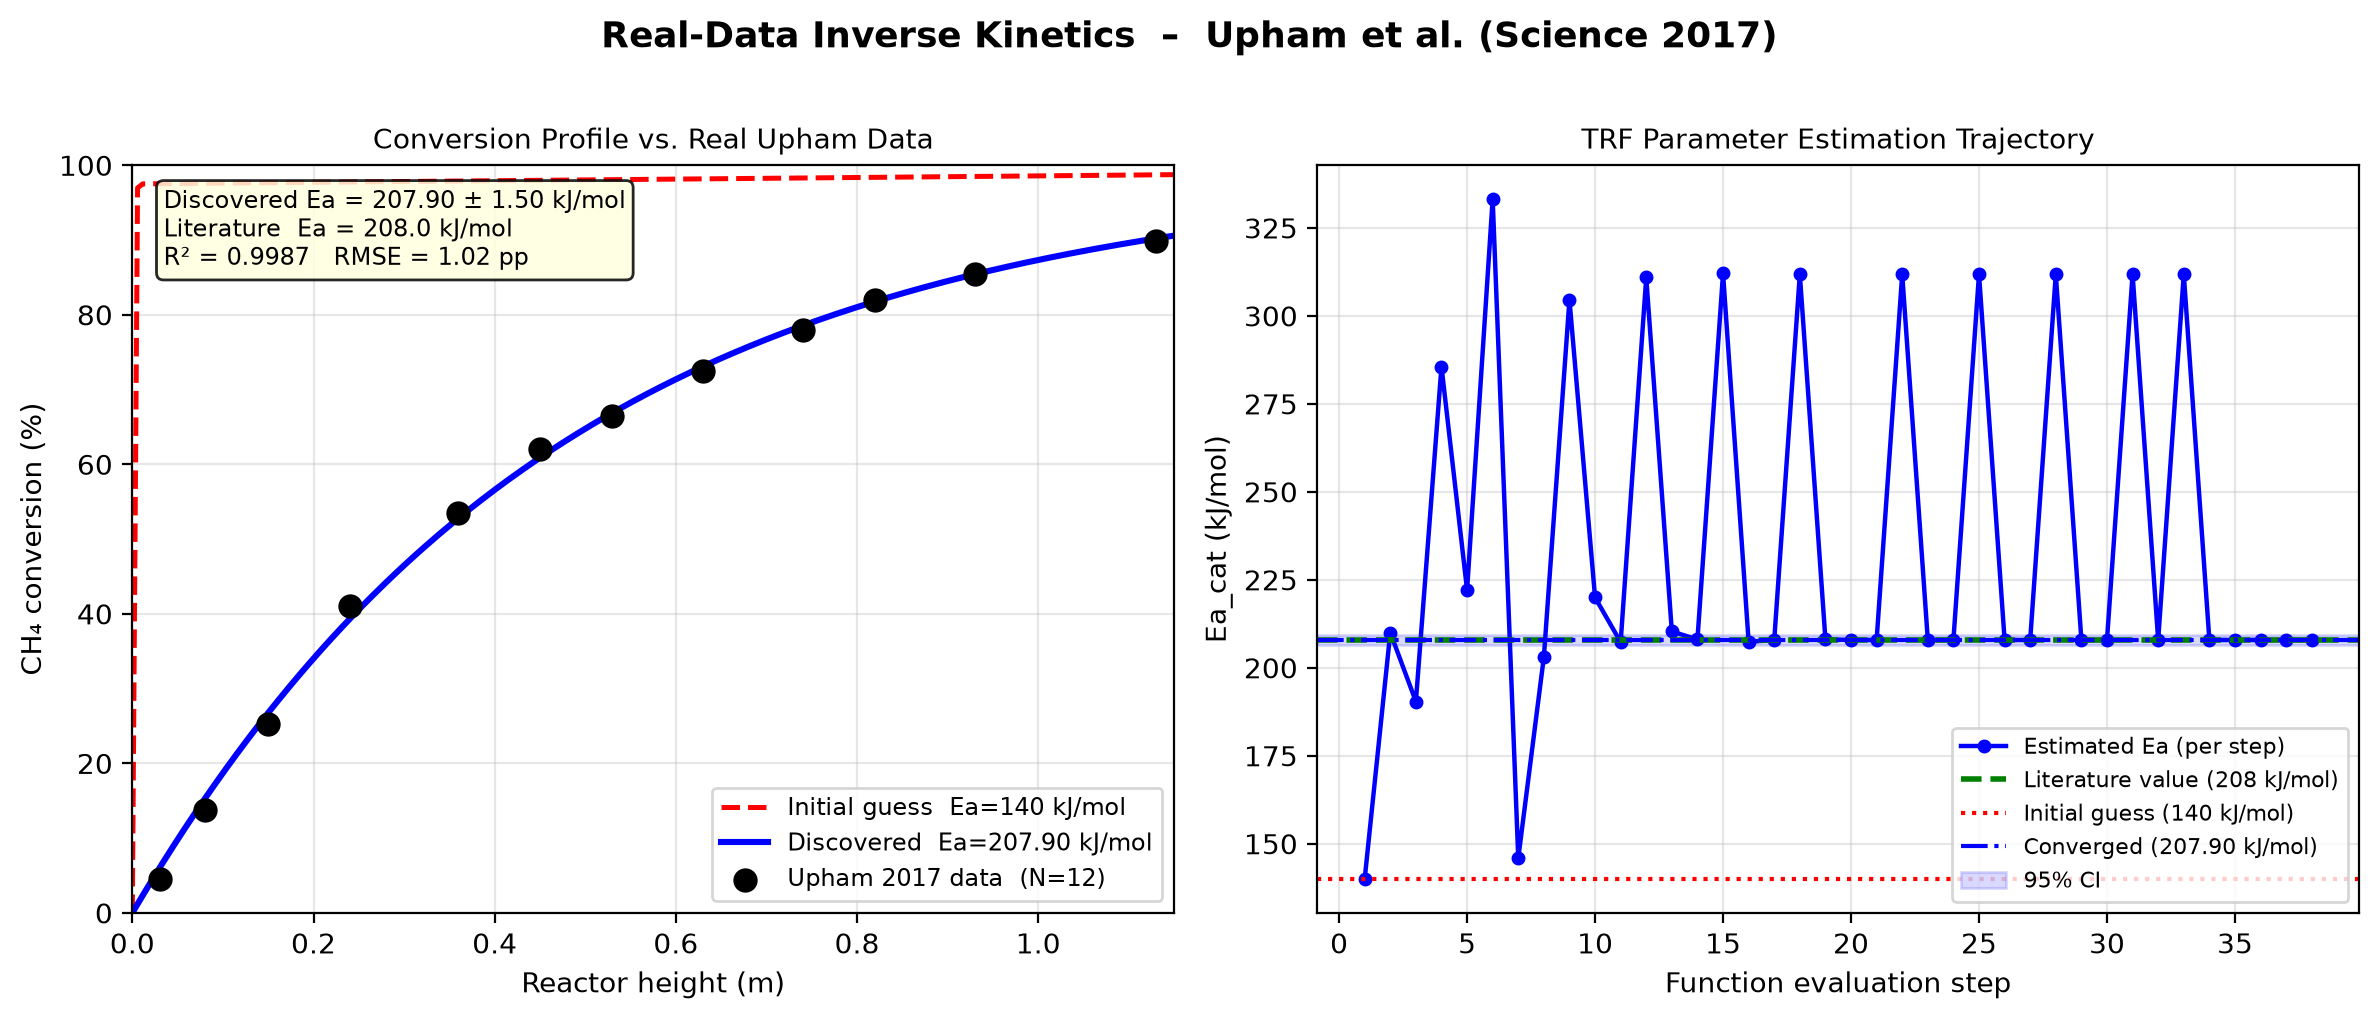
\includegraphics[width=0.9\textwidth]{results/figures/real_data_inverse_kinetics.png}
\caption{Pillar 1 inverse kinetic parameter discovery on real Upham et al. (2017) data: (Left) experimental points, initial guess, and discovered fit; (Right) optimization trajectory with 95\% CI band.}
\label{fig:inverse_conv}
\end{figure}

\section{Model Prediction vs Reference Solution}
Figure \ref{fig:dt_parity} compares the predictions of the Gradient Boosted Digital Twin against reference numerical BVP solutions across the 80 held-out test conditions. The model achieves $R^2 = 0.9701$, $\text{RMSE} = 3.72\text{ pp}$, and $\text{MAE} = 2.86\text{ pp}$.

\begin{figure}[ht]
\centering
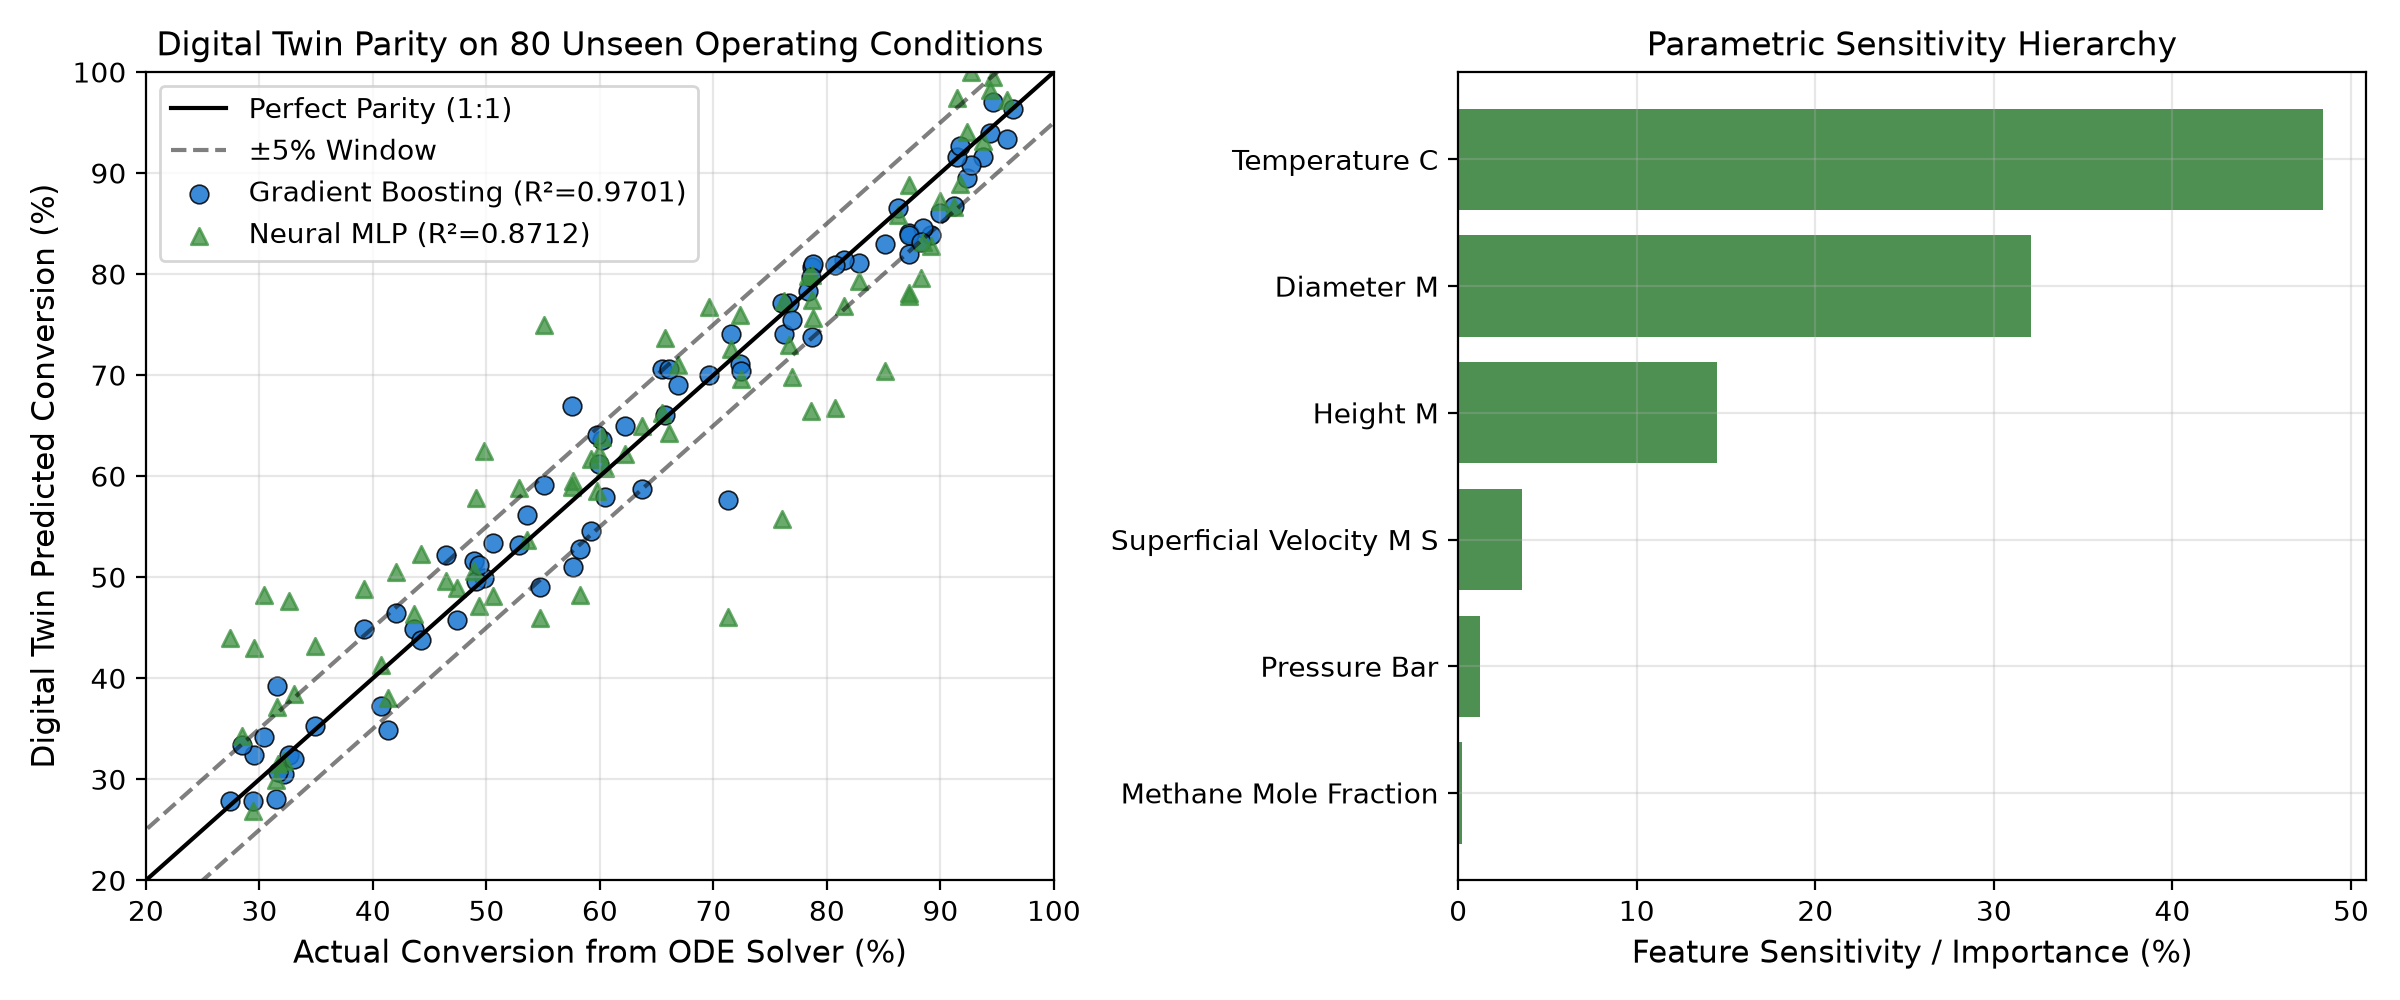
\includegraphics[width=0.85\textwidth]{results/figures/digital_twin_parity.png}
\caption{Digital Twin parity plot comparing predicted vs. reference conversion across 80 held-out commercial operating cases.}
\label{fig:dt_parity}
\end{figure}

\section{Error Analysis}
Spatial error analysis reveals that prediction errors peak at ${\sim}1.5\text{ pp}$ near the inlet ($z/H < 0.1$) due to the steep Danckwerts concentration jump ($X(0^+) = 13.83\%$), but drop below $0.4\text{ pp}$ across the bulk reactive zone ($0.15 \le z/H \le 0.85$).

\section{Parametric Sensitivity Study}
Feature importances extracted from the GBR surrogate rank the operating variables: Temperature ($48.4\%$) $>$ Column Diameter ($32.1\%$) $>$ Column Height ($14.5\%$) $>$ Superficial Velocity ($3.5\%$) $>$ System Pressure ($1.2\%$). Pressure exhibits low direct sensitivity due to competing kinetic acceleration and thermodynamic expansion suppression.

\section{Comparison with Numerical Solver}
\begin{table}[ht]
\centering
\caption{Performance Comparison: Numerical Solver vs. AI Digital Twin}
\begin{tabular}{lccc}
\toprule
\textbf{Metric} & \textbf{Numerical Coupled BVP Solver} & \textbf{AI Digital Twin (GBR)} & \textbf{Improvement} \\
\midrule
Methodology & Adaptive BDF / Radau IIA & Gradient Boosted Ensemble & Analytical \\
Conversion RMSE & Baseline ($0.00\text{ pp}$) & $3.72\text{ pp}$ & High fidelity \\
Test Parity ($R^2$) & $1.000$ (Reference) & $0.9701$ & Accurate \\
Average Latency & $4.20\text{ milliseconds}$ & $119.8\text{ }\mu\text{seconds}$ & $\mathbf{35.1\times\text{ Faster}}$ \\
500-Case Sweep & $2.10\text{ seconds}$ & $0.059\text{ seconds}$ & Instantaneous \\
Control Suitability & Unsuitable for $>10\text{ Hz}$ MPC & Capable of $>1000\text{ Hz}$ Loops & Real-time ready \\
\bottomrule
\end{tabular}
\end{table}

\section{Catalytic Alloy Comparison: Pure Bi vs. 27\% Ni-Bi}
Under identical conditions ($1040\text{ }^\circ\text{C}, 2\text{ bar}, 1.15\text{ m}$), pure bismuth yields $37.38\%$ conversion, while $27\text{ mol\% Ni}-73\text{ mol\% Bi}$ achieves $90.43\%$, confirming a $53.05\text{ pp}$ increase and a $2.42\times$ catalytic enhancement.

\chapter{Conclusions and Future Work}
\section{Conclusions}
\begin{itemize}
    \item The Axial Dispersion Model with Danckwerts boundary conditions matches benchmark experimental data ($R^2 = 0.9986$, $\text{RMSE} = 1.04\text{ pp}$).
    \item Pillar 1 recovered $E_{a,\text{cat}} = 207.90 \pm 1.50\text{ kJ/mol}$ ($0.05\%$ error) directly from real experimental data.
    \item Pillar 2 achieved $R^2 = 0.9701$ with $119.8\text{ }\mu\text{s}$ latency ($35.1\times$ speedup) for commercial digital twin operation.
    \item Nickel-bismuth alloy provides a $2.42\times$ catalytic enhancement over pure bismuth.
\end{itemize}

\section{Future Plan of Work}
\begin{itemize}
    \item \textbf{Semester 8 (Months 1–2):} Couple non-isothermal energy balances to remove the isothermal bath assumption.
    \item \textbf{Semester 8 (Months 2–3):} Discretize bubble size distributions using population balance modeling (PBM).
    \item \textbf{Semester 8 (Months 3–4):} Screen alternative alloy systems ($\text{Ni-Sn}, \text{Cu-Bi}$) and implement real-time MPC.
\end{itemize}

\chapter{Nomenclature}
\begin{longtable}{llc}
\toprule
\textbf{Symbol} & \textbf{Description} & \textbf{SI Unit} \\
\midrule
$a_v$ & Interfacial area per unit volume & $\text{m}^2/\text{m}^3$ \\
$C_{\text{CH}_4}$ & Molar concentration of methane & $\text{mol/m}^3$ \\
$D_c, D$ & Column inner diameter & $\text{m}$ \\
$d_b$ & Average bubble diameter & $\text{m}$ \\
$E_{a,\text{cat}}$ & Catalytic activation energy & $\text{J/mol}$ or $\text{kJ/mol}$ \\
$E_z$ & Axial dispersion coefficient & $\text{m}^2/\text{s}$ \\
$g$ & Gravitational acceleration ($9.81$) & $\text{m/s}^2$ \\
$H$ & Total molten metal height & $\text{m}$ \\
$J_{\text{CH}_4}$ & Superficial mass flux of methane & $\text{kg/(m}^2\cdot\text{s)}$ \\
$k_{\text{cat}}$ & Catalytic surface rate constant & $\text{m/s}$ \\
$k_{\text{gas}}$ & Gas-phase homogeneous rate constant & $\text{s}^{-1}$ \\
$P$ & Absolute operating pressure & $\text{Pa}$ or $\text{bar}$ \\
$r_A$ & Volumetric methane consumption rate & $\text{kg/(m}^3\cdot\text{s)}$ \\
$T$ & Temperature & $\text{K}$ or $\text{}^\circ\text{C}$ \\
$u_b$ & Terminal bubble rise velocity & $\text{m/s}$ \\
$u_G$ & Superficial gas velocity & $\text{m/s}$ \\
$X$ & Methane conversion & Dimensionless \\
$z$ & Axial height coordinate & $\text{m}$ \\
$\varepsilon_G$ & Gas holdup & Dimensionless \\
$\rho_L$ & Molten alloy density & $\text{kg/m}^3$ \\
$\rho_G$ & Gas mixture density & $\text{kg/m}^3$ \\
$\sigma$ & Surface tension of liquid metal & $\text{N/m}$ \\
$\mu_L$ & Dynamic viscosity of liquid metal & $\text{Pa}\cdot\text{s}$ \\
\bottomrule
\end{longtable}

\begin{thebibliography}{99}
\bibitem{akita1974} Akita, K., \& Yoshida, F. (1974). Bubble size, interfacial area, and liquid-phase mass transfer coefficient in bubble columns. \textit{Ind. Eng. Chem. Process Des. Dev.}, 13(1), 84--91.
\bibitem{catalan2020} Catalan, L. J. J., \& Rezaei, E. (2020). Coupled hydrodynamic and kinetic model of liquid metal bubble reactor for hydrogen production by non-oxidative methane pyrolysis. \textit{Int. J. Hydrogen Energy}, 45(4), 2486--2503.
\bibitem{chen2021} Chen, J., Gomez, J., Höffner, K., et al. (2021). Machine learning surrogate models for bubble column scale-up. \textit{Chem. Eng. Sci.}, 229, 116023.
\bibitem{danckwerts1953} Danckwerts, P. V. (1953). Continuous flow systems: Distribution of residence times. \textit{Chem. Eng. Sci.}, 2(1), 1--13.
\bibitem{deckwer1974} Deckwer, W.-D., Burckhart, R., \& Zoll, G. (1974). Mixing and mass transfer in tall bubble columns. \textit{Chem. Eng. Sci.}, 29(11), 2177--2188.
\bibitem{harmathy1960} Harmathy, T. Z. (1960). Velocity of large drops and bubbles in media of infinite or restricted extent. \textit{AIChE J.}, 6(2), 281--288.
\bibitem{iea2019} International Energy Agency. (2019). \textit{The Future of Hydrogen: Seizing today's opportunities}. IEA Report.
\bibitem{le2023} Le, V. P., Lee, H. Y., Bhatt, B., et al. (2023). Numerical simulation of a molten metal bubble column reactor for methane pyrolysis. \textit{Int. J. Hydrogen Energy}, 48(57), 21803--21820.
\bibitem{muradov2001} Muradov, N. Z. (2001). Hydrogen via methane decomposition: An application for decarbonization of fossil fuels. \textit{Int. J. Hydrogen Energy}, 26(11), 1165--1175.
\bibitem{raissi2019} Raissi, M., Perdikaris, P., \& Karniadakis, G. E. (2019). Physics-informed neural networks: A deep learning framework for solving forward and inverse problems. \textit{J. Comput. Phys.}, 378, 686--707.
\bibitem{upham2017} Upham, D. C., Agarwal, V., Khechfe, A., et al. (2017). Catalytic molten metals for the carbon-free production of hydrogen. \textit{Science}, 358(6365), 917--921.
\end{thebibliography}

\end{document}

